%- Use image processing algorithms in real-life problems
%- Each team member should investigate a separate issue/artifact/distortion
%- Dataset:
%    - Must collect your own data, in addition to existing datasets.
%- Method:
%    - For each issue/artifact/distortion, one must use at least two methods
%    - One of the methods must be a conventional image processing algorithm.
%      The other method could be either a conventional method or AI-based.
%    - Should modify existing methods to address issues in your collected dataset
%    - Feel free to use existing implementations
%- Comparison:
%    - Comparison with other methods, with and without the proposed method
%    - Discuss the results whether the proposed method improves the performance or not.

% Template for ICASSP-2026 paper; to be used with:
%          spconf.sty  - ICASSP/ICIP LaTeX style file, and
%          IEEEbib.bst - IEEE bibliography style file.
% --------------------------------------------------------------------------
\documentclass{article}
\usepackage{spconf,amsmath,graphicx,hyperref}
\usepackage{tikz}
\usetikzlibrary{arrows.meta}

% Example definitions.
% --------------------
\def\x{{\mathbf x}}
\def\L{{\cal L}}

% Title.
% ------
\title{Improving ID Card Scanning and Recognition: out of focus Blur and Specular Highlight removal}
%
% Single address.
% ---------------
\name{Aaryan Garg, Myles Lazarus}
\address{University of California, San Diego}

\begin{document}
%\ninept
%
\maketitle
%
\begin{abstract}
Smartphone-captured identity (ID) card images are frequently degraded by out of focus blur and specular highlights, which obscure characters and portrait details and cause errors in optical character recognition (OCR). We study both artifacts on ID-cards. For each artifact we compare a conventional method with a learning-based method: Wiener deconvolution with automatic blur-radius and noise estimation versus a pretrained transformer deblurring network, and a two-zone HSV-based method (inpainting of saturated highlight cores, veil correction of the unsaturated halo) versus a pretrained highlight-removal network. We adapt the methods to a self-collected dataset of paired, privacy-safe mock ID cards captured under controlled out of focus and glare conditions, in addition to public datasets. Methods are compared with and without our modifications and against unprocessed images using PSNR, SSIM, LPIPS, and OCR Character Error Rate (CER). % add video if we have time
\end{abstract}
%
\begin{keywords}
out of focus deblurring, specular highlight removal
\end{keywords}
%

% --------------------------------------------------------------------------
\section{Project objective}
\label{sec:objective}
% Summary of your project. Discuss the artifacts that you consider.
The objective of this project is to develop and evaluate an image-processing system that improves the quality of ID card images affected by two common acquisition artifacts: \textbf{out of focus blur} and \textbf{specular highlights} (glare). These artifacts frequently occur when ID cards are captured using smartphone cameras or document-scanning systems in both indoor and outdoor conditions.

out of focus blur occurs when the camera fails to focus accurately on the card, causing text and pictures to lose sharpness. Specular highlights occurs when light reflects from the card's laminated or glossy surface, producing bright regions that obscure the underlying information. Both artifacts can reduce the reliability of downstream tasks such as optical character recognition (OCR) and facial recognition.

The project investigates two restoration methods for each artifact: a conventional image-processing algorithm and a machine learning based approach. For out of focus blur, the methods are Wiener deconvolution and a pretrained deep-learning deblurring network. For specular highlights, the methods are a two-zone HSV-based approach (inpainting for saturated highlight cores and illumination-veil correction for the surrounding unsaturated halo) and a deep-learning highlight-removal network.

The project will use existing public research datasets where appropriate and collect additional images of ID-card-like documents under controlled and realistic conditions. The proposed algorithms will be adapted to the collected data and compared against unprocessed images and baseline methods. Performance will be evaluated using image-quality metrics, text-recognition accuracy, and visual inspection.

% --------------------------------------------------------------------------
\section{Introduction}
\label{sec:intro}
% Overview of the project and why it is important (broad impact).
% Discuss potential issues if the data is corrupted by the artifacts. Broad discussion of how you would solve the artifact issues.
Automated ID card scanning is increasingly important in banking, education, healthcare, travel, customer registration, and digital identity verification. These applications depend on the ability to extract information accurately from images of ID cards. However, taking pictures with cameras in practical environments introduces distortions that may hinder the extraction of relevant data.

out of focus blur reduces the contrast of edges and merges neighboring characters, making similar characters difficult to distinguish. For example, the characters “8” and “3” or “0” and “6” may become harder to separate. Specular highlights can completely saturate local image regions, concealing characters, portrait details, expiration dates, or other information. In severe cases, even a human observer cannot recover the original content from the captured image alone.

These problems can cause OCR errors, incorrect field extraction, failed verification, and repeated scanning attempts. Therefore, improving image quality before document analysis is an important practical computer-vision problem.

This project proposes a preprocessing and restoration pipeline that identifies the degradation type, applies a suitable correction method, and evaluates whether the restored image is more useful for subsequent document analysis. Conventional methods are attractive because they are computationally efficient and interpretable, while learning-based methods can learn complex image structures and degradation patterns. However, restoration must be performed carefully because aggressive processing can invent details, distort characters, or remove legitimate security features.

The project will therefore evaluate not only whether restored images look sharper or brighter, but also whether the restoration improves the accuracy of information extraction without introducing misleading visual content.

% --------------------------------------------------------------------------
\section{Literature review}
\label{sec:format}
% Literature review should include a broad review of both
% classical methods and ML methods for a particular artifacts. Then pick two
% methods with good performance (one should be classical method) that you plan to
% use for your artifact and give more detailed description of the methods.
\subsection{Out of focus blur}
An out of focused image is commonly modeled as $g = h \ast f + n$, where $f$ is the sharp image, $h$ the point spread function (PSF), and $n$, noise. For out of focus blur, $h$ is can be approximated as a uniform disk (or Gaussian) whose radius grows with the distance from the focal plane.

\textit{Classical methods.} Inverse filtering amplifies noise at frequencies where the PSF response is small; the Wiener filter~\cite{wiener1949,gonzalez2018} regularizes this using a noise-to-signal ratio and is the standard linear solution. Richardson--Lucy deconvolution~\cite{richardson1972,lucy1974} is an iterative maximum-likelihood alternative under Poisson noise. Prior-based methods use sparse gradient priors such as the hyper-Laplacian prior~\cite{krishnan2009}, and blind variants estimate the kernel jointly, e.g., with the dark channel prior~\cite{pan2016}. Text-specific priors exploit the near-binary nature of text~\cite{cho2012,pan2014}.

\textit{Learning-based methods.} Hradi\v{s} et al.~\cite{hradis2015} trained a CNN for direct text deblurring. General deblurring networks include DeblurGAN and DeblurGAN-v2~\cite{kupyn2018,kupyn2019}, SRN~\cite{tao2018}, and MPRNet~\cite{zamir2021}; recent efficient designs include Restormer~\cite{zamir2022} and NAFNet~\cite{chen2022}. out of focus-specific networks include the dual-pixel approach of Abuolaim and Brown~\cite{abuolaim2020} and IFAN~\cite{lee2021}, which predicts spatially adaptive filters. Learning-based methods generally yield higher PSNR/SSIM on benchmarks, but may hallucinate strokes on text, and generalize poorly to unseen blur types.

\textit{Selected methods.} We select (i) Wiener deconvolution as the conventional method, since a flat card held roughly parallel to the sensor yields a nearly uniform disk PSF, and (ii) Restormer~\cite{zamir2022} with weights trained for single-image out of focus deblurring as the learning-based method.

\subsection{Specular highlights}
\textit{What is specular reflection?}
Specular reflection is described by the dichromatic reflection model~\cite{shafer1985}: $I(\mathbf{p}) = m_d(\mathbf{p})\Lambda(\mathbf{p}) + m_s(\mathbf{p})$, i.e., a diffuse term (the true surface color) plus a specular term that carries the illuminant color. On laminated ID cards a highlight typically has two parts: a \emph{clipped core}, where the sensor saturates and the diffuse information is lost and can only be inferred from the surroundings, and a \emph{soft halo}, where the specular term is added on top of the diffuse signal without clipping, so characters are still present but with reduced contrast.

\textit{Classical methods.} Tan and Ikeuchi~\cite{tan2005} separate reflection components using chromaticity and a specular-free image. Yang et al.~\cite{yang2010} and Shen and Zheng~\cite{shen2013} give real-time methods based on bilateral filtering and intensity ratios. For saturated pixels, a common alternative is to detect a highlight mask and fill it by inpainting, e.g., Navier--Stokes~\cite{bertalmio2001}, fast-marching~\cite{telea2004}, or exemplar-based~\cite{criminisi2004} inpainting. Inpainting, however, synthesizes every masked pixel from its surroundings and discards whatever signal was already there, so it is inappropriate for the unsaturated halo. There, the glare acts as a smooth additive veil, which can be removed while keeping fine detail, e.g., by homomorphic or flat-field correction~\cite{gonzalez2018}, gradient-domain processing~\cite{perez2003}, or local contrast equalization such as CLAHE~\cite{zuiderveld1994}.

\textit{Learning-based methods.} Wu et al.~\cite{wu2021} built a real-world paired dataset for single-image highlight removal, and Fu et al.~\cite{fu2021} proposed a multi-task network that jointly detects and removes highlights, along with the SHIQ dataset. Most of these data consist of natural objects rather than flat printed documents, so domain shift is a concern.

\textit{Selected methods.} Because no single classical method handles both zones, we select (i) a two-zone conventional method that combines HSV-based highlight detection, fast-marching inpainting~\cite{telea2004} for the clipped core, and veil correction for the halo, and (ii) the multi-task network of Fu et al.~\cite{fu2021} as the learning-based method.

% --------------------------------------------------------------------------
\section{Artifacts and data collection}
\label{sec:pagestyle}
% Describe the artifacts that you are considering.
% Discuss how the artifacts might degrade the performance of the overall system.
% Discuss the dataset that you plan to use. Discuss your data collection plan.
\textbf{Artifacts.} \emph{out of focus blur} lowers edge contrast and merges adjacent glyphs; small fonts, dates, and machine-readable zones are the most affected. \emph{Specular highlights} saturate regions of the card and can hide complete fields or part of the portrait. Both reduce OCR accuracy and the reliability of face matching, and both are common when users hand-hold a phone near a glossy card.

\textbf{Public datasets.} We use MIDV-500, MIDV-2019, and MIDV-2020~\cite{arlazarov2019,bulatov2020,bulatov2022}, which contain mock ID documents captured on mobile devices, for OCR evaluation and as a source of sharp images. SmartDoc-QA~\cite{nayef2015} provides smartphone-captured documents with blur distortions. For learning-based baselines and sanity checks we use DPDD~\cite{abuolaim2020} and RealBlur~\cite{rim2020} for blur, and SHIQ~\cite{fu2021} for highlights.

\textbf{Own data collection.} To avoid privacy concerns we photograph \emph{mock} ID cards (fictitious names, numbers, and clip-art portraits, printed and laminated) and, with consent, redacted student cards. A smartphone is mounted on a tripod so that paired images share the same geometry. Table~\ref{tab:protocol} summarizes the protocol. Ground truth for out of focus is the in-focus photo; ground truth for glare is a photo under diffuse light. We also capture an unpaired hand-held set in uncontrolled indoor and outdoor settings, with ground-truth text transcribed manually, for realistic OCR evaluation. On the glare set we additionally label each text field as lying in a clipped core, in a soft halo, or outside the highlight, so that results can be reported per zone. We will also capture data which has both artifacts.

\begin{table}[t]
\centering
\small
\caption{Data collection protocol: a combination of the two artifacts will also be collected.}
\label{tab:protocol}
\begin{tabular}{p{0.5in}p{1.2in}p{1.2in}}
\hline
Factor & out of focus set & Glare set \\ % add combo
\hline
Cards & 10 mock cards, 2 layouts & same \\
Control & manual focus offset in 5--6 steps & lamp angle (3) $\times$ lamp distance (2) \\
Reference & in-focus pic & diffuse pic \\
Scenes & indoor, window, outdoor & same \\
Devices & $\geq$2 smartphones & $\geq$same \\
\hline
\end{tabular}
\end{table}

% --------------------------------------------------------------------------
\section{Proposed Approach}
\label{sec:typestyle}
% Describe your approach and how it can improve
% performance. Provide details. Use block diagrams and figures.
Fig.~\ref{fig:pipeline} shows the overall system. A lightweight assessment stage computes the variance of the Laplacian (blur indicator) and the fraction of near-saturated, low-chroma pixels (glare indicator), and routes the image to the appropriate branch. In each branch, the conventional and learning-based outputs are compared with the unprocessed image using image-quality metrics and OCR.

\begin{figure}[t]
\centering
\resizebox{\columnwidth}{!}{%
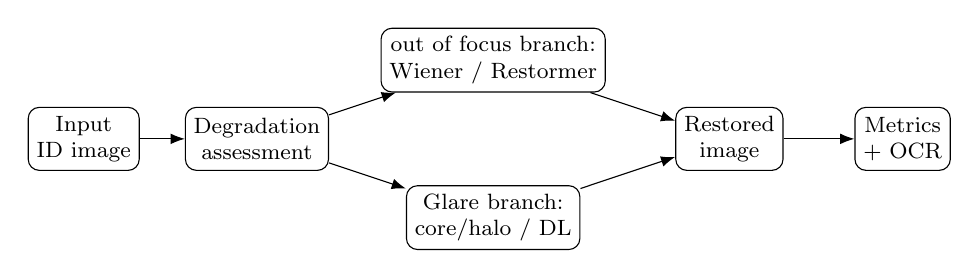
\begin{tikzpicture}[
  box/.style={draw,rounded corners,align=center,minimum height=8mm,font=\footnotesize,inner sep=3pt},
  arr/.style={-{Latex[length=1.8mm]}}]
\node[box] (in) at (0,0) {Input\\ID image};
\node[box] (qa) at (2.2,0) {Degradation\\assessment};
\node[box] (b)  at (5.2,1.0) {out of focus branch:\\Wiener / Restormer};
\node[box] (g)  at (5.2,-1.0) {Glare branch:\\core/halo / DL};
\node[box] (out) at (8.2,0) {Restored\\image};
\node[box] (ev) at (10.4,0) {Metrics\\+ OCR};
\draw[arr] (in) -- (qa);
\draw[arr] (qa) -- (b);
\draw[arr] (qa) -- (g);
\draw[arr] (b) -- (out);
\draw[arr] (g) -- (out);
\draw[arr] (out) -- (ev);
\end{tikzpicture}}
\caption{Overview of the proposed restoration and evaluation pipeline.}
\label{fig:pipeline}
\end{figure}

\subsection{Out of focus blur}
\textbf{Conventional: adapted Wiener deconvolution.} The Wiener filter in the frequency domain is
\begin{equation}
\hat F(u,v) = \frac{H^{*}(u,v)}{|H(u,v)|^{2} + K}\, G(u,v),
\end{equation}
where $K \approx \sigma_n^2/\sigma_f^2$. Using it as-is requires a known PSF and $K$, so we modify it for our data as follows:
\begin{enumerate}
\item \emph{Luminance processing.} Deconvolve only the luminance channel to avoid color fringes.
\item \emph{Automatic PSF radius.} Model $h$ as a disk of radius $R$. We sweep $R$ over a candidate range, deblur, and choose the $R$ that maximizes a score combining normalized gradient sharpness and mean OCR word confidence. A ringing penalty prevents over-sharpening.

\item \emph{Noise-adaptive $K$.} Estimate $\sigma_n$ from the median absolute deviation of the finest wavelet band, approximate the signal variance as $\sigma_f^2 \approx \max(\operatorname{Var}(g)-\sigma_n^2,\epsilon)$, and set $K = \lambda \sigma_n^2/\sigma_f^2$, where $\lambda$ is a global scale tuned on a validation split.

\item \emph{Boundary handling.} Apply edge tapering before the FFT to suppress border ringing.
\end{enumerate}
\textbf{Learning-based: Restormer.} We run the pretrained out of focus-deblurring Restormer~\cite{zamir2022} with tiled inference for high-resolution inputs. We then fine-tune it with a small learning rate and $L_1$ loss on (a) paired real captures and (b) synthetic pairs created by blurring sharp frames from MIDV with random disk radii and noise, and compare the pretrained and fine-tuned versions.

\subsection{Specular highlights}
\textbf{Conventional: two-zone highlight removal.} A highlight consists of a clipped core and an unsaturated halo (Sec.~\ref{sec:format}). Inpainting the entire mask would replace recoverable low-contrast text in the halo with synthesized content, so we treat the zones differently:

let $V=\max(R,G,B)$ and $S=(V-\min(R,G,B))/V$

\begin{enumerate}
\item \emph{Clipped seeds.}
Identify pixels with very high intensity through a threshold on the least bright color $\min(R,G,B)\ge\tau_c$ to form the set $C$. These would form islands (seeds) on the image, and the ones smaller than $A_{\min}$ pixels are removed as noise. If no seeds remain, the image is passed through unchanged.
\item \emph{Hysteresis growth.} Estimate the normal card brightness $B$ and its spread $\sigma_B$ as the standard deviation of $V$ over the card image, excluding $C$. The low threshold is $\tau_l = B + k\sigma_B$ (e.g., $k=3$), i.e., a pixel is ``abnormally bright'' relative to the card. Starting from $C$, repeatedly add neighboring pixels with $V>\tau_l$ and $S<\tau_s$ (since glare is nearly white), up to a distance $r_{\max}$ from the seeds. The result is the full highlight region $M \supseteq C$.
\item \emph{Component filtering.} Discard components of $M$ whose area exceeds $A_{\max}$ which indicates a blank region rather than a local highlight.
\item \emph{Zone split.} The core is $M_c = C$. The halo is $M_h = M \setminus M_c$.
\item \emph{Core: inpainting.} Fill each component of $M_c$ using fast-marching inpainting~\cite{telea2004}. Components larger than an area limit are flagged as unrecoverable so the system can request recapture and avoid imaginary content.
\item \emph{Halo: veil correction.} In $M_h$ the glare is modeled as a smooth additive veil. We estimate it as a low-pass feature, subtract it, and increase contrast. Gradient-domain correction~\cite{perez2003} and CLAHE~\cite{zuiderveld1994} serve as alternatives.
\item \emph{Blending.} Feather the boundary between zones to avoid visible seams, which can create false edges for OCR.
\end{enumerate}
The parameters ($\tau_c$, $k$, $\tau_s$, $A_{\min}$, $A_{\max}$, $r_{\max}$, and the kernel size of the veil low-pass) are tuned on a split of our collected data.
\textbf{Learning-based: multi-task network.} We apply the pretrained detection-and-removal network of Fu et al.~\cite{fu2021} and fine-tune it on our paired glare set with $L_1$ and perceptual losses. We also measure agreement between its predicted mask and our HSV mask (IoU) to analyze detection quality.

\textbf{Combined Artifacts}
For images containing both out-of-focus blur and specular highlights, we apply both restoration methods sequentially, comparing deblurring followed by highlight removal against the reverse order. We evaluate both sequences using OCR accuracy and image-quality metrics to determine which ordering produces better results.

\textbf{Evaluation.} For each artifact we compare: unprocessed input, the conventional method, and the learning-based method pretrained and fine-tuned. On paired data we report PSNR, SSIM~\cite{wang2004}, and LPIPS~\cite{zhang2018}. On all data we run Tesseract~\cite{smith2007} (and optionally a second OCR engine) and report character error rate (CER), word error rate, and field-level accuracy, together with runtime. Qualitative inspection checks for hallucinated or distorted characters and for damage to security features. For glare we measure error rates separately for each zone: clipped core, and low contrast halo. PSNR/SSIM are additionally computed inside $M$. We also compare the application of deblurring before highlight removal and vice-versa.

% --------------------------------------------------------------------------
\section{Discussion}
\label{sec:majhead}
% Discuss any potential issues that you might face
\textbf{Data.} Aligning paired captures is difficult; small shifts penalize PSNR/SSIM, so we use a tripod and image registration. Mock cards are not identical to real ones, and the dataset is small, which limits fine-tuning and generalization. Real IDs involve privacy and consent issues.

\textbf{Blur.} Real out of focus is not perfectly uniform: a tilted card gives a spatially varying PSF, and phone cameras add processing, noise, and compression that violate the linear model. Wiener deconvolution may produce ringing or amplify noise, whereas deep models may hallucinate characters that look plausible but are wrong, which is dangerous for identity verification.

\textbf{Glare.} Saturated pixels contain no information about the original content, so in the core any method can only guess. Conversely, inpainting is harmful where contrast survives, which motivates the two-zone design, but the boundary between ``clipped'' and ``recoverable'' is not sharp and depends on the camera's exposure and tone mapping; its threshold must be tuned on our data and may not transfer to other devices. Veil correction assumes a smooth additive glare and can fail when the glare has sharp edges, and feathering can leave residual seams. HSV rules may misclassify white background, hologram, or laminate features, and both inpainting and veil correction can alter real security patterns. Deep models trained on natural-object datasets may transfer poorly to documents.

\textbf{Evaluation.} OCR results depend on the engine and on image resolution; PSNR/SSIM may not match OCR gains. We therefore report several metrics and test more than one OCR engine.

\textbf{Stretch goals} 1) We can potentially extend this to ID card scanning from video data instead of just images. That can potentially lead to better recovery of data by combining information across frames. 2) Also, along with OCR, we can also further evaluate performance on facial recognition tasks for IDs that have the picture of the ID owner as well. 3) Another future study which can be done for highlight removal is a hybrid approach where the highlight detection is done using a CNN but the removal is still done using classical methods. 4) For deblurring, it can be extended to other types of blur such as motion blur etc.

% To start a new column (but not a new page) and help balance the last-page
% column length use \vfill\pagebreak.
% -------------------------------------------------------------------------
%\vfill
%\pagebreak

% References should be produced using the bibtex program from suitable
% BiBTeX files (here: strings, refs, manuals). The IEEEbib.bst bibliography
% style file from IEEE produces unsorted bibliography list.
% -------------------------------------------------------------------------
\bibliographystyle{IEEEbib}
\bibliography{strings,refs}

\end{document}
